\section{Introduction}
This chapter outlines the process for evaluating the system, describing a field study in a naturalistic environment 
\section{Field Study - Observation of The System In a Natural Environment}
\subsection{Outline \& Objectives}
The primary purpose of our study is to identify the contribution of gamification on the system: whether it improves or hinders user engagement \& enjoyment. To quantify the value of gamification in the system, we use an A/B Testing~\cite{ABTesting} approach. This involves comparing two near-identical versions of the system with the exception of a single variation, allowing us to measure the impact of said variation on user behaviour. As such two systems were implemented \textbf{`System A' (without gamification)} and \textbf{`System B' (with gamification)}. 

\subsection{Study Methodology}
There exist two applicable methods to evaluate our system, laboratory and field studies. We can define a laboratory study as:
\begin{quotation}
\noindent
`A research study conducted in a contrived setting in which the effect of all, or nearly all, influential but irrelevant independent variables is kept to a minimum.''~\cite[p.~215]{marketStudy}
 \end{quotation}

Lab experiments are preferable in situations where the environment and variables need to be controlled. The outcome of this method is data specific to what you want to test. On the other hand, the controlled surroundings may ignore not reflect the use of the system in a wider general context.

Oppositely, a field study is:
\begin{quotation}
\noindent
``A research study conducted in a natural setting in which one or more independent variables are manipulated by the experimenter under conditions controlled as carefully as the situation will permit.''\cite[p. 211]{marketStudy}
 \end{quotation}

The advantage of a field study is the ability to test the system in a natural environment, allowing us to deal with the exact same environment where the system would be used. On the other hand, we have less control of the external variables, which may introduce `confounding variables'\footnote{Confounding variables directly or indirectly link the dependant and independent variables.} that can negative affect the studies external validity~\cite{fieldstudysux}.

\subsubsection{Selected method}
A field study was selected as we want to see how a novel way of collecting loyalty stamps works in the real world. We can see how users learn to use the system throughout the study. Not having control of the environment can prove advantageous as we can isolate and attempt to remediate any negative variables that are caused by `natural use'. A pilot study (to be discussed in Sec. xx) will need to be performed in order to identify some of these initial variables.

\subsection{Demographics}
Six participants were recruited that owned a compatible Android device (Android 4.4 KitKat+) for our system. An even amount of male and females were recruited eventhough women tend to frequent loyalty schemes more often than men~\cite{womenloyalty}. All participants were students within our target demographic of 16-40, having the average age of 21.5.

\subsection{Preparation}
Two systems were prepared for the study --- `System A' (without gamification) and `System B' (with gamification). The primary functionality of both systems are identical except for the addition of badges/quests to System B. Participants were evenly assigned a system to test at random. We required users to install the application on their own device to ensure the system works with a variety of hardware. 

An example loyalty scheme `Bath Cafe' was setup for the study (Fig. \ref{fig:bathcafe}). It was designed in such a way that users will be able to claim at a free coffee by the end of the study.

\begin{figure}[H]
 \centering
  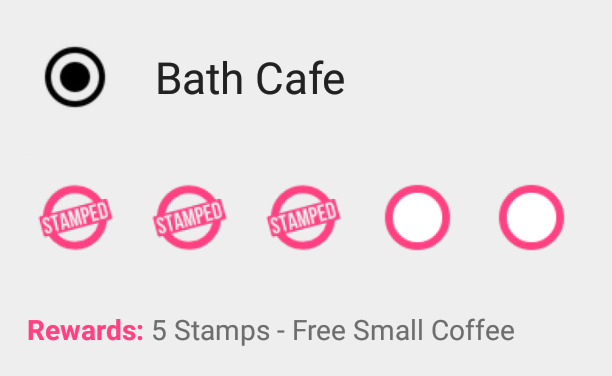
\includegraphics[width=0.40\textwidth]{img/bathcafe.png}
     \caption{The example loyalty scheme to be used in the study. A reward of a free coffee is offered upon completing the stamp card.}
     \label{fig:bathcafe}
\end{figure}

An accompanying badge was created for the loyalty scheme, as can be seen in Fig. \ref{fig:badge2}. The badge was purposefully simple to collect in order to be attainable throughout the study.

\begin{figure}[H]
 \centering
  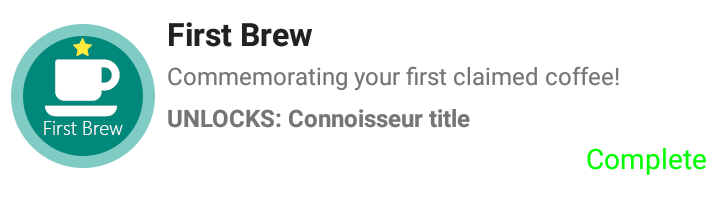
\includegraphics[width=0.50\textwidth]{img/badge2.png}
     \caption{A badge implemented for the study. Both the badge and the `connoisseur' title unlock when a user claims their first coffee.}
     \label{fig:badge2}
\end{figure}
 
Three coffee shop locations were identified on a university campus to perform the field study. A random location was to be visited on each of the five days. At each location a business employee will be asked to use the `Stamped Manager' application to facilitate our study.
 
\subsection{Developing The Questionnaire}
The primary method of gathering quantitative data from this study is using a questionnaire, complimented by some comment questions to gather further qualitative data for their answers.

We prepared two questionnaires, one for the participants to complete upon finishing the study and one for a coffee shop employee to fill-out at every unique location visited for the study. An explanation of their purpose follows:

\subsubsection{Questionnaire For Users}
The user questionnaire attempts to quantify the participant's loyalty scheme patterns and their response to the application and technology. To achieve this, the questionnaire was broken down into several sections.
\begin{itemize}
	\item \emph{Questions 2 \& 3} informs a participants behaviour regarding loyalty schemes. Having a wide variety of loyalty scheme behaviours allow us to get a complete range of opinions regarding our system.
	\item \emph{Question 4} was introduced from the Technology Acceptance Model (TAM)~\cite{tam} (Fig. \ref{fig:TAM}). The TAM models how individuals accept and use new technology based on `perceived usefulness' and `perceived ease of use' factors--- satisfying these variables predicts a system that is more likely to see use~\cite{tam}.
	\item \emph{Question 5} one way in which we can gauge how much participants enjoyed using the system is to identify whether the participant would recommend the system to friends. Furthermore, personal use also indicates system enjoyment.  
	\item \emph{Questions 6 \& 7} Are specific to the tested system, only one of them requiring an answer. By asking these questions, we aim to understand what potential impact, positive or negative, gamification can have on the system. 
	\item \emph{Question 8} Requires users to provide qualitative feedback about their experience. We ask for positives and negatives in order to encourage a balance in the answers, along with suggestions for system improvements.
\end{itemize}

Whereas question 4 is designed to measure user trust in the system (whether users will use the system), questions 5, 6 and 7 are to be used to measure our hypothesis.

\begin{figure}[H]
 \centering
  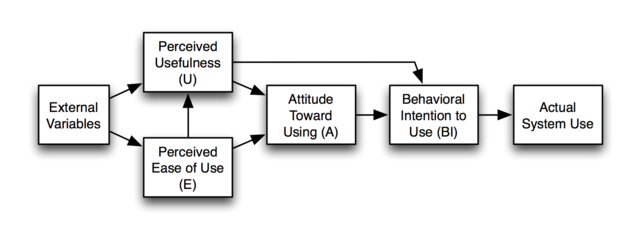
\includegraphics[width=0.80\textwidth]{img/TAM.png}
     \caption{The Technology Acceptance Model (TAM) modelling the link `perceived usefulness' and `perceived ease of use' has on system use }
     \label{fig:TAM}
\end{figure}

\subsubsection{Questionnaire For Business}
The business questionnaire is designed to give context to the location where a field study is being performed. The questions mainly identify what type of loyalty schemes exist within that business, the rewards they give and the percentage of customers that participate in them. Finally there is an option for employees to provide feedback on the Stamped Manager. Effort was made to keep this questionnaire as simplistic as possible to ensure minimum disturbance of the employees.

\subsection{Pilot Study}
A pilot study allows the identification of correct processes and captures any small issues that may affect the primary field study. The primary purpose of the pilot is to assess the interaction using the application on a participant's phone.

A separate participant was recruited. She described limited-to-no knowledge of mobile technologies and was a casual consumer of smartphones. They were told to download and install Stamped, whilst we installed the Stamped Manager on a tablet device. A list of tasks was generated in order to test the `interaction elements' (stamping/reward claiming) of the applications. In the interest of time, we designed the tasks to be completed in one sitting.

The list of tasks were as follows:

\begin{enumerate}
  \item Login to the system using your university email and password `1234`
  \item Ensure your phone is unlocked (you do not need to have the application open) to collect a stamp
  \item Tap your phone onto the reader when asked (you will be given 5 stamps)
  \item Click on the notification/open the application
  \item Ensure you received 5 stamps in the loyalty scheme `Bath Cafe`
  \item Swipe to the profile page
  \item Confirm that you have 1 available reward on your profile page
  \item Swipe to the rewards tab
  \item Select the available reward `free coffee`
  \item Notify the researcher that you want to claim a reward
  \item Tap your phone onto the reader when asked
  \item Open swipe to your schemes and ensure the stamps have been deducted
\end{enumerate}

\paragraph{Findings}

The user was proficient at navigating the application, a tabbed interface proved to be easy for them to understand. Several user interface bugs were also quickly discovered, such as no feedback when a user tries to login with incorrect credentials. These were corrected before the main study took place.

Some questions on the questionnaire were deemed to be confusing and had to be revised for the future study. 

Various hardware-level issues were identified that intruded with the interaction. Different phones have their NFC Chip located in various places, making it difficult to know where users should tap their device. There were points where they were sliding the back of their phone on the tablet in attempt to trigger the interaction. Moreover, we identified that using a very thick protective `phone-case' (as the participant had), limited some NFC signal.

Positioning the tablet on the stand was a problem. The stand put the device at an awkward angle on table with regards to the user, making it difficult to tap the back of the device with a smartphone. Furthermore the awkward angle sometimes caused a `weak NFC interaction'\footnote{A weak NFC interaction occurs when an NFC interaction is interrupted mid-way, thus one device fails to communicate its message, whilst the other believes it has taken place.}, providing unintended feedback that would trick users into thinking that an interaction has occurred.

\paragraph{Solutions}

As a majority of the issues were hardware orientated, several process solutions were implemented to remediate them for the main study. Firstly for future participants, we checked if their phone-case was not too thick, asking them to remove it for the purpose of the study if necessary. Secondly they were instructed to `swipe' along the back of the tablet instead of a simple tap to ensure the NFC interaction completes. 

The ideal solution for this problem would be to purchase a USB-to-MicroUSB adapter and a standalone USB NFC reader for the Stamped Manager (Fig. \ref{fig:usbnfc}), having the user tap their smartphone on the reader instead. Using this configuration will not only correct the awkward angle/weak interaction problem, but will also provide NFC functionality to devices that do not have it available.  The flexibility of this solution would make it preferrable for businesses.

\begin{figure}[H]
 \centering
  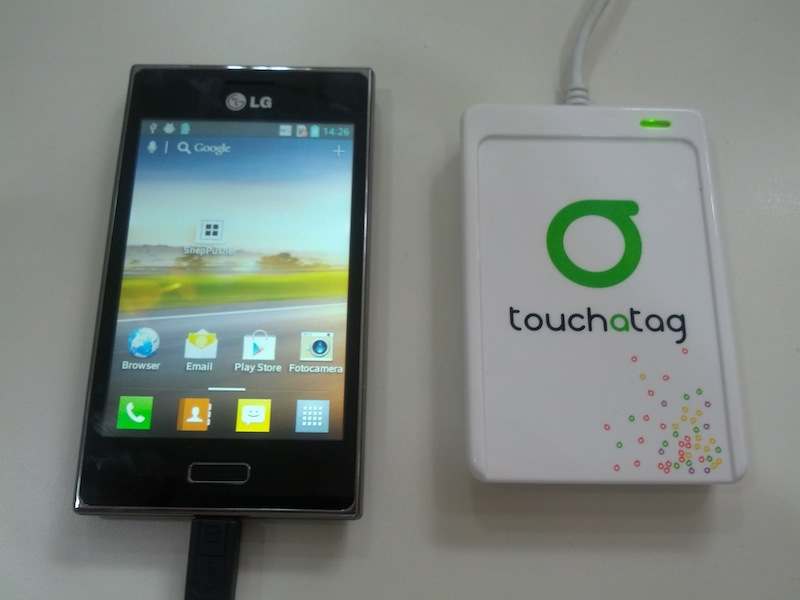
\includegraphics[width=0.4\textwidth]{img/nfcusb.jpg}
     \caption{A smartphone device connected to a USB NFC reader}
     \label{fig:usbnfc}
\end{figure}

\subsection{Hypothesis}
We clarify our hypothesis to be expanded on as \textbf{Hypothesis A: Participants using Gamification are more likely to enjoy to system and recommend it to friends}. We understand that `enjoy' is a very general term, and therefore attempt to quantify this by using questions 5, 6, 7 in our questionnaire as our dependant variables (Fig. \ref{fig:questionz}). Those with gamification should respond more positively to Q5 than those without. Moreover, participants should respond positively to the question unique to their system (Q6 or Q7).
\begin{figure}[H]
 \centering
  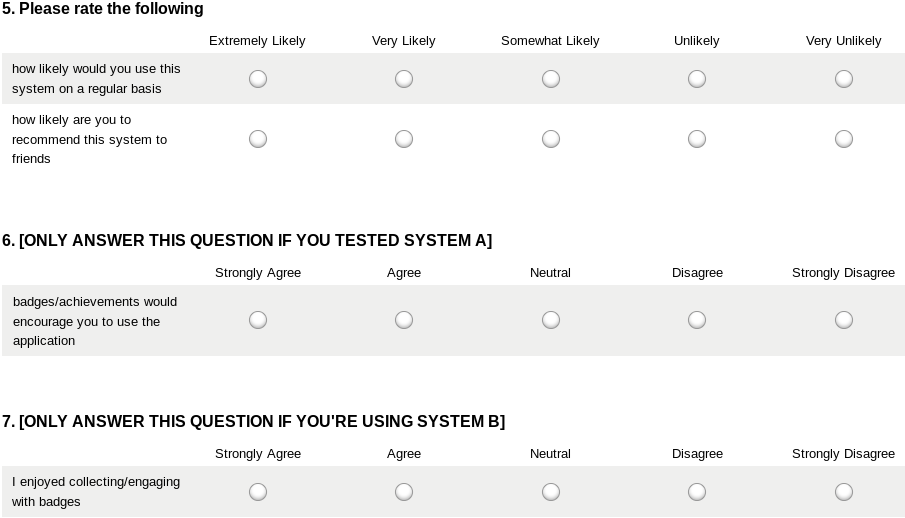
\includegraphics[width=0.81\textwidth]{img/questions.png}
     \caption{Questions 5, 6, 7 of our questionnaire to be used as our dependant variables}
     \label{fig:questionz}
\end{figure}
\newpage
\subsection{Approach}
Here we describe the process by which the study was performed. The researcher began by briefing the participants as per Fig. XXX on the context and purpose of the project. They were guaranteed that the system is being tested rather than themselves, along with the confidentiality in their responses by storing no personally identifying information. Participants were then required to download and install their assigned system onto their smartphones (Fig. \ref{fig:fieldstudyfamily}) --- instructions can be found in appendix XXX. Finally, they were asked to sign a permission slip, an example of which can be seen in Sec. XXX.

The main directive given to the participants is that they must collect stamps throughout the study, claiming a free coffee once they have accumulated enough of them. Those testing System B (with gamification) were directed to ensure that they collect the badge by the end of the study. 

\begin{figure}[H]
 \centering
  \includegraphics[width=0.60\textwidth]{img/fieldstudyfamily.png}
     \caption{A photograph showing the three devices which used System B}
     \label{fig:fieldstudyfamily}
\end{figure}

We began the study by setting a convenient time to meet everyday in an earlier communicated coffee shop for the session. It was important to select a non-peak time as to minimise disturbance to the staff. All six participants were sat down and asked to wait; meanwhile the researcher asks the coffee shop employee to use the tablet with the Stamped Manager  for the next six people that ask for a `digital stamp'. They were assured that the stamps were only for a study and not legible --- this was followed by a quick training on how to use the Stamped Manager. The tablet was left on the till, ready for the employee to use to distribute stamps.
\newpage
Once training was completed, the participants were instructed to travel individually to perform a regular coffee shop transaction, claiming a digital stamp (or free coffee) from the employee. The interaction was two-way; employees have to press the appropriate button on the Manager (Stamp/Receive Reward), whilst the participants swipe their phone onto the back of the tablet (Fig. \ref{fig:hollystamping}). Meanwhile, the researcher sat down to observe the interactions between them. At the end of each session, the researcher would ask the employee to fill in the business questionnaire. Once all formal parts of the session were complete, participants were offered a cupcake for their troubles.

\begin{figure}[H]
 \centering
  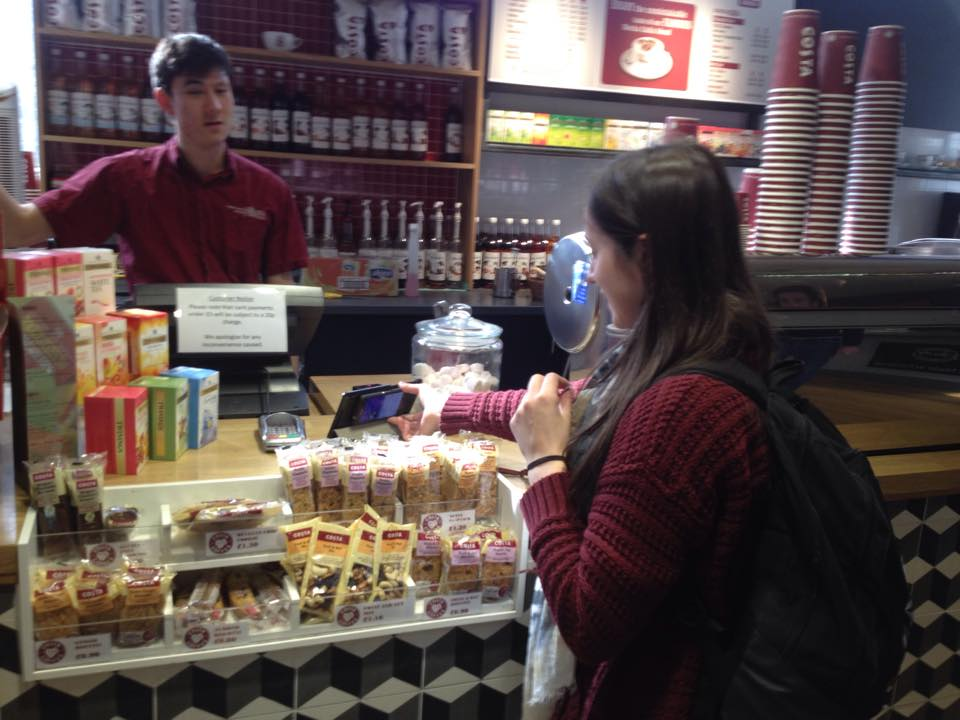
\includegraphics[width=0.6\textwidth]{img/hollystamping.jpg}	
     \caption{An photograph of the field study - a participant is seen claiming a stamp at the counter of a coffee shop}
     \label{fig:hollystamping}
\end{figure}

This format was repeated every day for five consecutive days (Monday-Friday), with each session lasting 10-20 minutes. By the end of the study, participants should have tested all three main interactions (stamping, reward claiming and badge receiving). Finally, upon confirming that all participants have completed their tasks, the post-study questionnaire was disseminated for them to complete.
 
\section{Conclusion}
This chapter outlined how our field study was conducted, along with the elements which we are trying to quantify. In the next chapter, we will discuss the findings of the study.